\documentclass[a4paper]{article}

\usepackage{INTERSPEECH2021}

% Put the lab number of the corresponding exercise
\title{NLU course project}
\name{Gianluigi Vazzoler (257846)}

\address{
  University of Trento}
\email{gianluigi.vazzoler@studenti.unitn.it}

\usepackage{graphicx}
\usepackage{subcaption} % For subfigure environment
\graphicspath{{plots/}}

% Ottimizzazioni per ridurre gli spazi
\usepackage{float}
\setlength{\textfloatsep}{0pt plus 0pt minus 0pt}
\setlength{\floatsep}{0pt plus 0pt minus 0pt}
\setlength{\intextsep}{0pt plus 0pt minus 0pt}
\setlength{\abovecaptionskip}{3pt}
\setlength{\belowcaptionskip}{3pt}

\begin{document}

\maketitle

% ──────────────────────────────────────────────────────────────────────────────
% SEZIONI IN DUE COLONNE (template INTERSPEECH2021)
% ──────────────────────────────────────────────────────────────────────────────

\section{Introduction}
This report describes the modifications made to a baseline RNN model to improve its performance on a language modeling task. The goal was to reduce the perplexity on the validation set by implementing various architectural changes and optimization techniques. The modifications included replacing the RNN with an LSTM, adding dropout layers, switching to AdamW optimizer, implementing weight tying, using variational dropout, and applying non-monotonic averaged SGD (NT-AvSGD) for better generalization. The results demonstrate significant improvements in perplexity over the baseline.

\section{Implementation details}
Starting from the provided RNN baseline, we implemented two main stages of modifications to improve perplexity on the given dataset:

\subsection{Part 1.A}
\begin{itemize}
  \item \textbf{LSTM Replacement:} Replaced the original vanilla RNN cell with a single‐layer LSTM while keeping the same data loader and training loop.
  \item \textbf{Dropout:} Added two dropout layers—one after the embedding layer and another just before the final output projection.
  \item \textbf{Optimizer Switch:} Switched from SGD (tuned over \{1.0, 2.0\}) to AdamW (tuned over \{0.0005, 0.001, 0.002\}).
\end{itemize}
Each configuration was trained for up to 100 epochs with early stopping if validation perplexity did not improve for five epochs.

\subsection{Part 1.B}
\begin{itemize}
  \item \textbf{Weight Tying:} The input embedding and output projection share the same weight matrix so that each word uses a single representation when read and when predicted. This reduces parameters and improves generalization.
  \item \textbf{Variational (Locked) Dropout:} During training, each example uses one fixed dropout pattern over the entire sequence rather than changing at every time step. We also sometimes mask out entire word vectors for the full forward pass. This stabilizes learning and provides consistent regularization.
  \item \textbf{NT‐AvSGD (Non‐Monotonic Averaged SGD):} We tracked the best validation perplexity and, whenever the validation score worsened compared to earlier epochs (ignoring the most recent few), started averaging model parameters over subsequent epochs instead of choosing a single checkpoint. Averaging after validation stops improving yields a smoother final model that generalizes better.
\end{itemize}
Each run lasted up to 100 epochs, and NT‐AvSGD was triggered automatically based on validation checks.

All modifications were implemented by following \cite{Merity18-ROC}.

\section{Results}
The evaluation uses perplexity (PPL) to assess how well the model predicts sequences — lower PPL means better performance. Tables 1 and 2 summarize the results from experiments in Part 1.A and 1.B. Figure 1 and 2 show the best‐performing configuration for each experiment of part A, while Figure 3 does the same but for part B. Eventually, Figure 4 explores how the best runs from both parts compare against each other.

\subsection{Architectures}
Replacing the vanilla RNN with an LSTM led to a significant reduction in perplexity, confirming the effectiveness of gating mechanisms in addressing gradient vanishing. The best results were achieved with the model that combined LSTM, weight tying, variational dropout, and NT-ASGD, which consistently outperformed simpler configurations.

\subsection{Regularisation}
Applying variational (locked) dropout provided a consistent improvement across models, particularly in terms of generalisation. By stabilising the hidden dynamics during training, this technique helped reduce overfitting and produced more stable validation performance.

\subsection{Optimisation Strategy}
The transition from standard SGD to AdamW already yielded initial gains, especially when tuning learning rates appropriately. However, the most substantial improvement came from NT-ASGD, which adaptively averaged model parameters after stagnation in validation scores. This method proved particularly effective when combined with other regularisation strategies.

\subsection{Learning Rate Sensitivity}
Extensive hyperparameter tuning highlighted the critical role of learning rate selection. For AdamW, a learning rate of approximately 0.001 consistently yielded stable and effective convergence. In contrast, NT-AvSGD achieved optimal performance with learning rates between 2.0 and 4.0, with the best results observed at 4.0. However, increasing the learning rate beyond this range sometimes led to training instability.

\bibliographystyle{IEEEtran}
\bibliography{mybib}

% ──────────────────────────────────────────────────────────────────────────────
% DA QUI IN POI: PASSAGGIO A COLONNA SINGOLA
% ──────────────────────────────────────────────────────────────────────────────
\onecolumn

% ──────────────────────────────────────────────────────────────────────────────
% TABELLE E FIGURE OTTIMIZZATE PER L'USO DELLO SPAZIO
% ──────────────────────────────────────────────────────────────────────────────

\begin{table}[H]
  \centering
  \caption{Part 1.A results. The best results for each architecture are highlighted in \textbf{bold}.}
  \label{tab:final_results_1a}
  % \vspace{-3pt}      % <<< rimosso: non serve se non ci sono figure subito dopo
  \begin{tabular}{llllrrr}
    \toprule
    Architecture & Optimizer & LR & Dropout(p) & PPL / Dev & PPL / Test & Epochs \\
    \midrule
    RNN  & SGD   & 0.5 & /   & \textbf{164.68} & \textbf{155.71} & 29 \\
    RNN  & SGD   & 1.0 & /   & 170.04          & 161.68          & 14 \\
    RNN  & SGD   & 2.0 & /   & 185.32          & 175.88          & 9  \\
    \midrule
    LSTM & SGD   & 0.5 & /   & 149.75          & 143.31          & 31 \\
    LSTM & SGD   & 1.0 & /   & \textbf{148.58} & \textbf{141.76} & 23 \\
    \midrule
    LSTM & SGD   & 1.0 & 0.3 & 129.71          & 124.91          & 99 \\
    LSTM & SGD   & 2.0 & 0.3 & \textbf{127.82} & \textbf{122.73} & 51 \\
    \midrule
    LSTM & AdamW & 0.001 & 0.3 & 124.61       & 113.70          & 32 \\
    LSTM & AdamW & 0.001 & 0.4 & \textbf{119.33} & \textbf{107.62} & 50 \\
    LSTM & AdamW & 5e-4  & 0.4 & 122.64       & 110.14          & 58 \\
    LSTM & AdamW & 0.005 & 0.4 & 120.20       & 108.25          & 50 \\
    \bottomrule
  \end{tabular}
\end{table}

\vspace{6em}

\begin{table}[H]
  \centering
  \caption{Part 1.B results. The best results for each architecture are highlighted in \textbf{bold}.}
  \label{tab:part1b_sorted}
  % \vspace{-3pt}      % <<< rimosso: non serve se non ci sono figure subito dopo
  \begin{tabular}{llllllrrr}
    \toprule
    Architecture &  Optimizer  &  LR & Dropout(p) &  PPL / Dev &  PPL / Test &  Epochs \\
    \midrule
    LSTM + weight tying & SGD      & 0.5 & /   & 125.45 & 122.96 & 46 \\
    LSTM + weight tying & SGD      & 1.0 & /   & \textbf{120.79} & \textbf{118.81} & 31 \\
    \midrule
    LSTM + weight tying + variational dropout & SGD      & 1.0 & 0.3 & 99.34 & 96.58 & 100 \\
    LSTM + weight tying + variational dropout & SGD      & 2.0 & 0.4 & \textbf{97.67} & \textbf{94.98} & 100 \\
    \midrule
    LSTM + weight tying + variational dropout & NT-AvSGD & 2.0 & 0.4 & 98.96 & 95.09 & 100 \\
    LSTM + weight tying + variational dropout & NT-AvSGD & 3.0 & 0.4 & 96.07 & 91.59 & 100 \\
    LSTM + weight tying + variational dropout & NT-AvSGD & 4.0 & 0.4 & \textbf{95.67} & \textbf{91.14} & 100 \\
    \bottomrule
  \end{tabular}
\end{table}

\vspace{6em}

% <<< da qui inizia la modifica più sostanziale:

% === Parte 1.A plots: dividiamo la figura in due blocchi ===

% 1) Primo blocco: subfigure (a) e (b) subito sotto Tabella 2
\begin{figure}[H]
  \centering
  \begin{subfigure}[b]{0.48\textwidth}
    \centering
    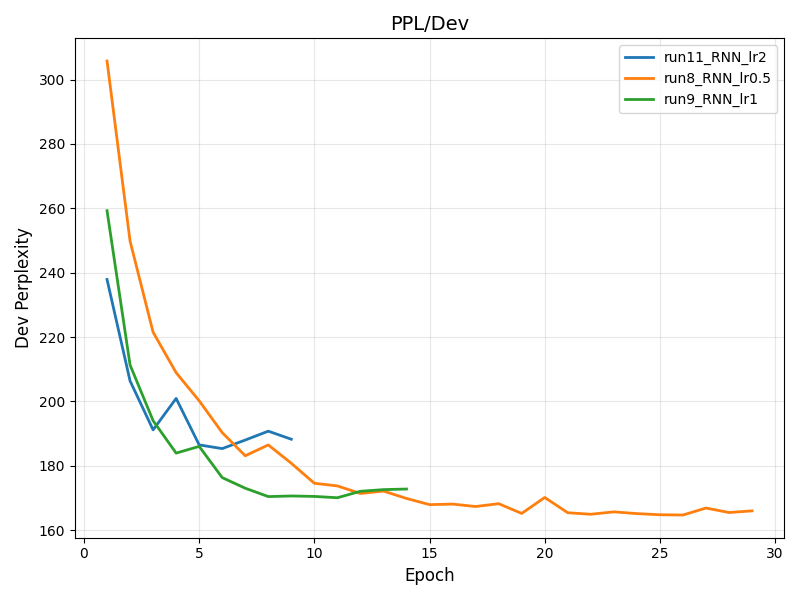
\includegraphics[width=\textwidth]{RNN_plot.png}
    \caption{RNN — SGD 0.5 vs 1.0 vs 2.0}
    \label{fig:rnn_plot}
  \end{subfigure}
  \hfill
  \begin{subfigure}[b]{0.48\textwidth}
    \centering
    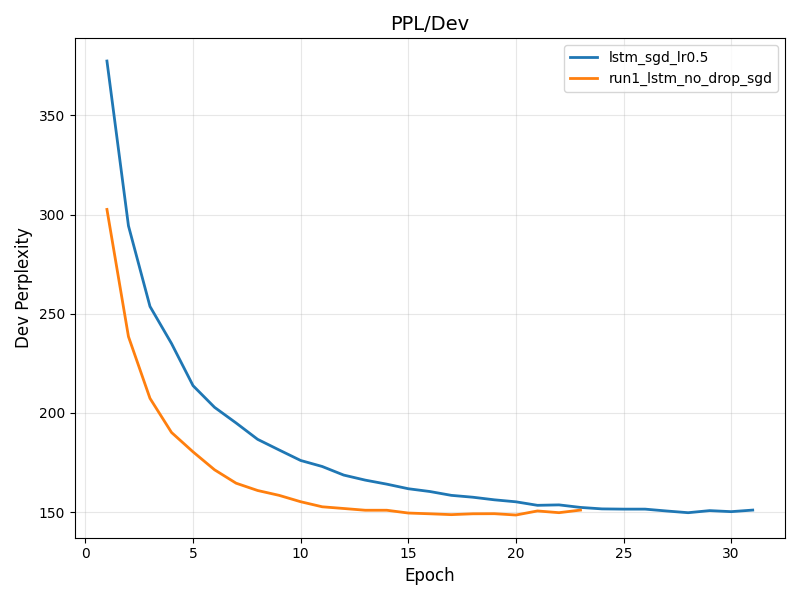
\includegraphics[width=\textwidth]{LSTM_plot.png}
    \caption{LSTM — senza dropout, SGD 0.5 e 1.0}
    \label{fig:lstm_plot}
  \end{subfigure}
  \caption{Perplexity vs Epochs trends (Part 1.A, first two plots).}
  \label{fig:plots_part1a_prima_riga}
\end{figure}

% Forziamo nuova pagina per il secondo blocco (se non c’è più spazio, LaTeX già lo farà,
% ma un \clearpage aiuta a eliminare bianchi vuoti imprevedibili)
\clearpage

% 2) Secondo blocco: subfigure (c) e (d) nella pagina seguente
\begin{figure}[H]
  \centering
  \begin{subfigure}[b]{0.48\textwidth}
    \centering
    % qui il terzo plot di Part 1.A
    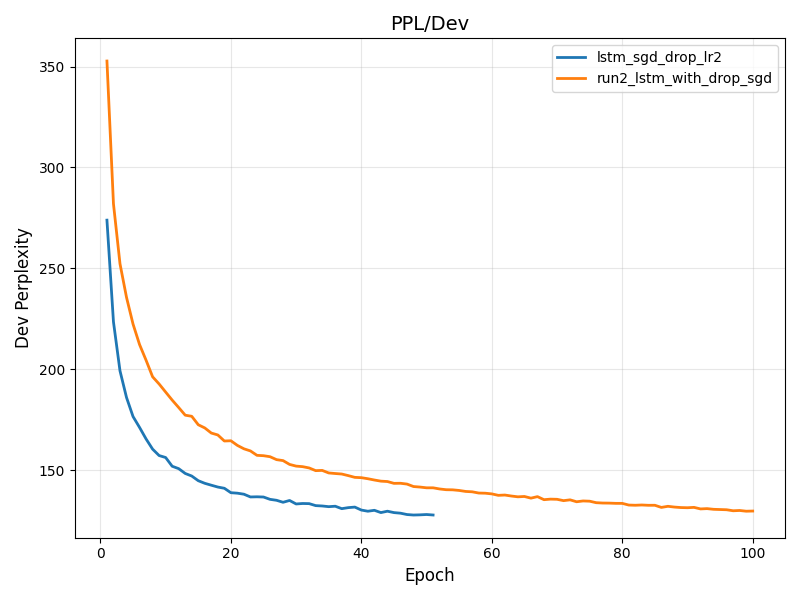
\includegraphics[width=\textwidth]{LSTM_drop_plot.png}
    \caption{LSTM + Dropout — SGD 1.0 e 2.0}
    \label{fig:lstm_drop_plot}
  \end{subfigure}
  \hfill
  \begin{subfigure}[b]{0.48\textwidth}
    \centering
    % qui il quarto plot di Part 1.A
    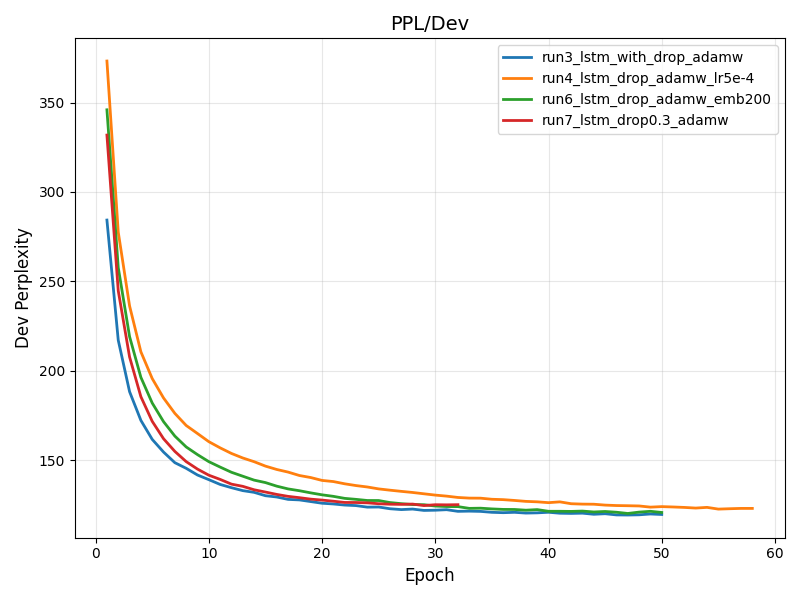
\includegraphics[width=\textwidth]{LSTM_drop_adamw_plot.png}
    \caption{LSTM + Dropout + AdamW}
    \label{fig:lstm_drop_adamw_plot}
  \end{subfigure}
  \caption{Perplexity vs Epochs trends (Part 1.A, last two plots).}
  \label{fig:plots_part1a_seconda_riga}
\end{figure}

% <<< fine modifica Parte 1.A

\vspace{2pt}

% Part 1.B plots - layout ottimizzato
\begin{figure}[H]
  \centering
  \begin{subfigure}[b]{0.49\textwidth}
    \centering
    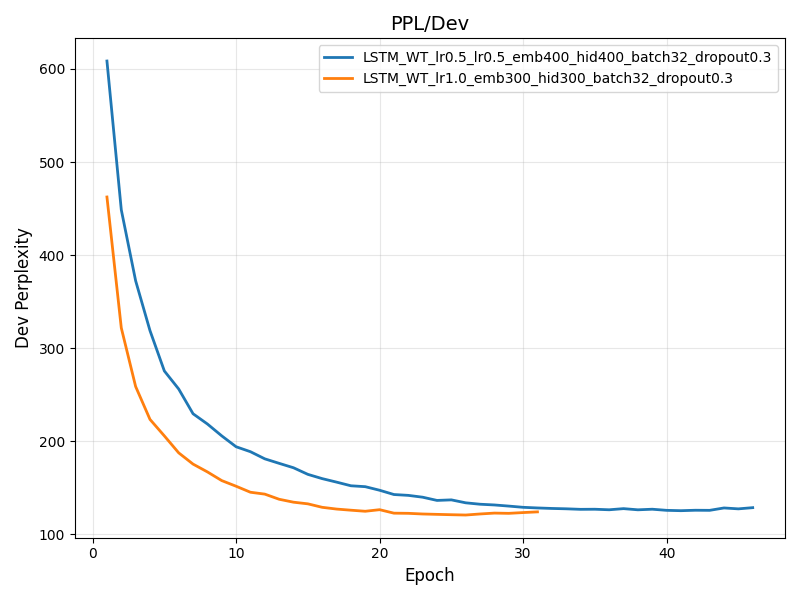
\includegraphics[width=\textwidth]{LSTM_WT_plot.png}
    \caption{LSTM + Weight Tying (SGD 0.5 vs 1.0)}
    \label{fig:lstm_wt_plot}
  \end{subfigure}
  \hfill
  \begin{subfigure}[b]{0.49\textwidth}
    \centering
    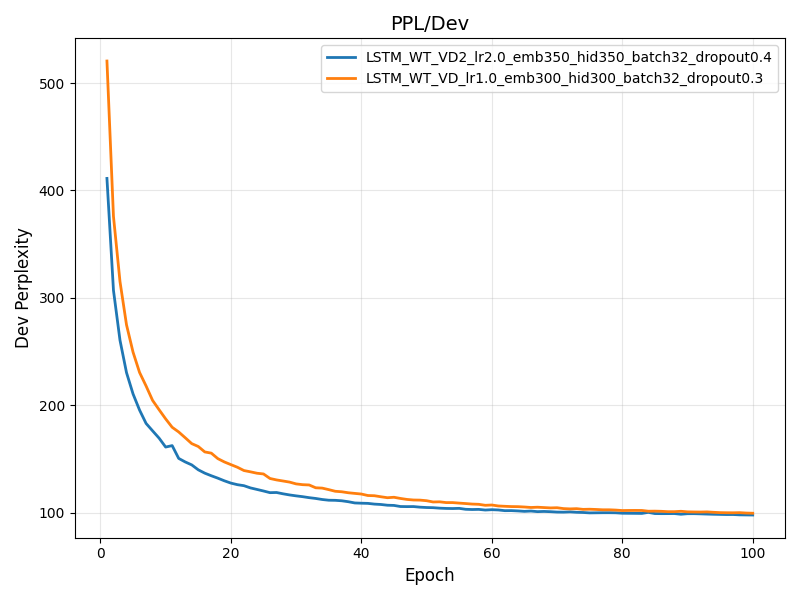
\includegraphics[width=\textwidth]{LSTM_WT_VD_plot.png}
    \caption{LSTM + WT + Variational Dropout (SGD 1.0 vs 2.0)}
    \label{fig:lstm_wt_vd_plot}
  \end{subfigure}
  
  \vspace{8pt}
  
  \begin{subfigure}[b]{0.6\textwidth}
    \centering
    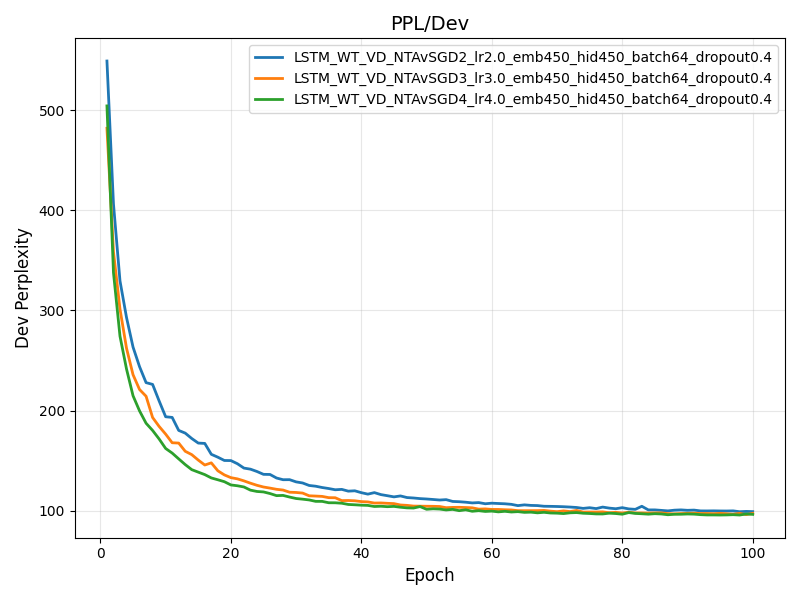
\includegraphics[width=\textwidth]{LSTM_WT_VD_NTAvSGD_plot.png}
    \caption{LSTM + WT + VD + NT-AvSGD (lr 2.0, 3.0, 4.0)}
    \label{fig:lstm_wt_vd_ntasgd_plot}
  \end{subfigure}
  
  \caption{Perplexity vs Epochs trends for the configurations in Part 1.B.}
  \label{fig:plots_part1b}
\end{figure}

\vspace{-10pt}

% Plot finale ottimizzato
\begin{figure}[H]
  \centering
  \vspace{-5pt}
  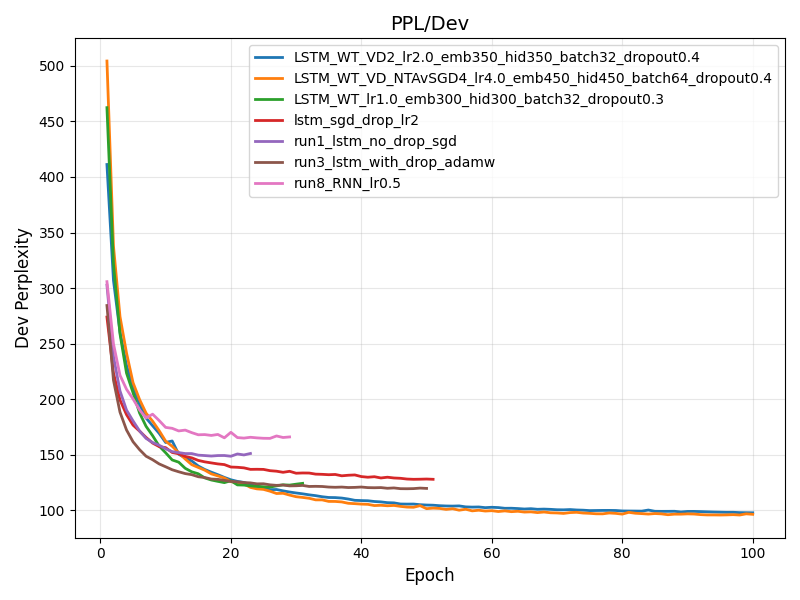
\includegraphics[width=0.75\textwidth]{best_runs_plot.png}
  \vspace{-3pt}
  \caption{Comparison of the "best runs" (in bold) from both Part 1.A and Part 1.B.}
  \label{fig:best_runs}
\end{figure}

\vspace{-10pt}

\end{document}
